\chapter{Kombinatorische Schaltungen}

Unter Kombinatorischen Schaltungen versteht man elektrische Schaltungen aus mehreren Logikgattern.
Diese findet man unter Anderem in einem Prozessor und sind die elementaren Bausteine der Logik eines Computers.

\begin{Ziele} 
In diesem Kapitel lernst du ...
\begin{itemize}
\item wie Logikgatter aus Transistoren aufgebaut sind,
\item die Grundlagen der Aussagenlogik,
\item welche Darstellungsformen es für logische Schaltungen gibt,
\item wie man von einer Problemstellung zu einer funktionierenden Schaltung gelangt,
\item wie man logische Schaltungen verkürzen und minimalisieren kann,
\item wie ein Computer mit Logikgattern addieren kann.
\end{itemize}
\end{Ziele}


\section{Logikgatter aus Transistoren}

In Abschnitt \ref{Sec:Logikgatter} haben wir bereits Ersatzschaltbilder zu den Logikgattern angegeben.
Diese bestanden jedoch noch aus gewöhnlichen Schaltern statt aus Transistoren.
Nun werden wir die Logikgatter durch Transistoren beschalten lassen.


\begin{Aufgabe} \label{Aufg:Logikgatter}
Implementiere in \textsc{Yenka} die folgenden drei Transistorschaltungen. Den \emph{Logic Indicator} findest du unter Lab Equipement $\Rightarrow$ Logic. 
\begin{center}
\begin{tabular}{ccc}
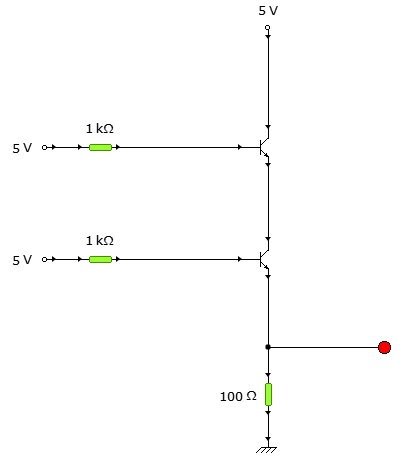
\includegraphics[scale=.4]{pics/ANDTrans}
&
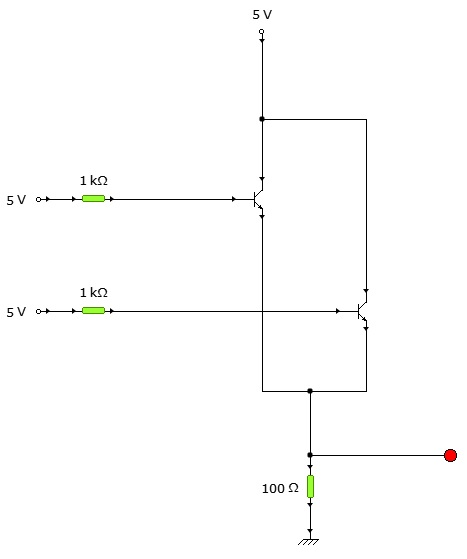
\includegraphics[scale=.4]{pics/ORTrans}
&
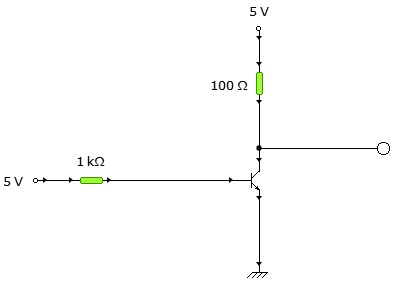
\includegraphics[scale=.4]{pics/NOTTrans}
\\
(a) & (b) & (c)
\end{tabular}
\end{center}

Die Spannungen links stellen jeweils die Eingangsspannung dar. Die Spannung oben stellt die Versorgungsspannung dar. Unten ist jeweils die Masse (der Minuspol). Rechts zeigt der \emph{Logic Indicator} an, ob hohe (1) oder niedrige (0) Spannung angelegt ist.


Implementiere die Schaltungen in \textsc{Yenka} und teste diese, indem du die Eingangsspannungen veränderst (0 oder 1). Gib an, um welches Logikgatter es sich jeweils handelt.

Übernimm die Schaltungen in dein Heft!
\end{Aufgabe}

Im folgenden wird geklärt, warum die Transistorschaltungen wie die entsprechenden Logikgatter funktionieren.

Beginnen wir bei (a). Mache dir Stichpunkte darüber in dein Heft.
Dafür benötigen wir die Spannungsteilerregel. 
Die Versorgungsspannung von $5V$ (ganz oben) fällt bis zur Masse (ganz unten) vollständig ab.
Über jedem Widerstand auf dieser Strecke fällt dabei etwas dieser $5V$ ab.
Je größer ein Widerstandswert, desto mehr Spannung fällt über diesen ab.

Sind nun beide Eingänge auf 1 (links), werden die beiden Transistoren mit hoher Spannung angesteuert.
Dadurch haben beide Transistoren einen sehr kleinen Widerstand.
Über beiden Transistoren fällt demnach nur sehr wenig Spannung ab.
Der Rest der Spannung muss also am unteren Widerstand abfallen ($300 \Omega)$.
Demzufolge ist zwischen dem Transistor und dem unteren Widerstand, also dort, wo wir die Spannung mit dem \emph{Logic Indicator} messen, eine hohe Spannung zu finden (1).
Kurz gesagt: Sind beide Eingänge auf 1, ist auch der Ausgang auf 1.

Ist allerdings mindestens ein Eingang auf 0, liefert also wenig Spannung an den entsprechenden Transistor, dann hat dieser Transistor einen riesigen Widerstand.
Das bedeutet, über diesem Transistor fällt der Hauptteil der Versorgungsspannung ab.
Hinter beiden Transistoren ist dann nur sehr wenig Spannung vorhanden.
Der \emph{Logic Indicator} liegt demnach auf 0.

All diese Beobachtungen kannst du auch in \textsc{Yenka} sehen, wenn du mit der Maus auf ein Bauelement gehst. Beobachte die Spannungswerte am Eingang und am Ausgang der Widerstände.


\begin{Aufgabe} \label{Aufg:OrMasche}
Untersuche auf die gleiche Weise, warum die Schaltung in (b) wie ein OR-Gatter arbeitet! Mache dir Stichpunkte dazu in dein Heft! Dafür solltest du den Maschensatz (Abbildung \ref{Abb:Maschensatz}) noch einmal wiederholen.
\end{Aufgabe}

\begin{Zusatzaufgabe}
Untersuche auf die gleiche Weise, warum die Schaltung in (c) wie ein NOT-Gatter arbeitet!
\end{Zusatzaufgabe}

\begin{Aufgabe} \label{Aufg:NANDNORTransistor}
Implementiere auf gleiche Weise das NAND- und das NOR-Gatter als Transistorschaltung. Das NAND-Gatter stellt dabei die Negation des AND-Gatters dar (NOT AND). Das NOR-Gatter ist die Negation des OR-Gatters (NOT OR). Dabei kannst du durch Kombination der obigen Schaltungen darauf kommen. Es gibt aber auch je eine Lösung, die nur zwei Transistoren benötigt!
\end{Aufgabe}

\begin{Aufgabe} \label{Aufg:NANDNORTerm}
Gib für das NAND- und das NOR-Gatter eine Schalttabelle und einen logischen Term an!
\end{Aufgabe}



%\begin{Aufgabe} \label{Aufg:Gatter}
%Öffne im Tauschordner die Datei \emph{LogikStart.yka} und implementiere eine Schaltung aus zwei Transistoren und einer LED, die
%\begin{itemize}
%\item[(a)] Wie ein AND-Gatter funktioniert
%\item[(b)] Wie ein OR-Gatter funktioniert
%\item[(c)] Wie ein NOT-Gatter funktioniert
%\end{itemize}

%Dabei sollen die Eingangswerte an die jeweiligen Emitter angeschlossen werden.
%Den Ausgangswert kannst du bestimmen, indem du an der entsprechenden Stelle einen \emph{Logic Indicator} (Lab Equipement $\Rightarrow$ Logic) anschließt. Ist die Spannung auf 1, dann leuchtet er, ist die Spannung auf 0 bleibt er weiß.
%\end{Aufgabe}



In der Realität stellt das NAND-Gatter das wichtigste der Gatter dar.
Denn im Prozessorbau werden nur NAND-Gatter verwendet.
In der Tat kann man jedes Gatter durch ein NAND-Gatter ersetzen (auch wenn man teilweise mehrere NAND-Gatter braucht um bspw. das AND-Gatter darzustellen).
In der Praxis ergeben sich dadurch dennoch Kostenersparnisse, da man nur ein Gatter produzieren muss.



\section{Kombinationen der Gatter}

\textbf{Hinweis:} In Schaltungen, die aus Logikgattern bestehen, lässt man üblicherweise Spannungsquellen und Versorgungsspannungen weg. Für eine sogenannte \emph{logische Schaltung} werden demnach nur die Logikgatter, Eingänge (in Form von Schaltern) und einen Ausgang (oder mehrere Ausgänge) benötigt.

Obwohl es nicht danach aussieht, handelt es sich dennoch um einen Gleichstromkreis.

\begin{Aufgabe}
\hfill \par \vspace*{-.8cm}
\begin{itemize}
\item[(a)]
Gegeben ist die Funktionsdarstellung einer Schaltung mit:
\begin{align*}
(a \wedge b) \wedge c
\end{align*}
Lege eine Schaltbelegungstabelle an und implementiere die Schaltung in \textsc{Yenka}!

\textbf{Hinweise:} Logikgatter befinden sich in \textsc{Yenka} unter Electronic Components $\Rightarrow$ Digital Processing $\Rightarrow$ Digital 4000 Series $\Rightarrow$ Logic Gates. Stelle mit Rechtsklick $\Rightarrow$ Properties $\Rightarrow$ Electronics $\Rightarrow$ Appearance auf Logic Levels und Use IEC Logic Symbols um! \\
Für die Eingänge bietet sich unter Lab Equipment $\Rightarrow$ Logic die Latching Logic Inputs an, für den Ausgang der Logic Indicator, ebenda.
\item[(b)] Gib eine Schaltbelegungstabelle an und implementiere die Schaltung: $(a \vee b) \vee c$
\item[(c)] Wofür stehen die Klammern? Was passiert am Ausgang, wenn man stattdessen $a \wedge (b \wedge c)$ implementiert?
\end{itemize}
\end{Aufgabe}


Um eine Schaltung aus mehreren Gattern zu implementieren, muss man aus dem logischen (oder mathematischen) Term die Reihenfolge der Verarbeitung der Signale erkennen.

Dabei gilt die folgende Reihenfolge der Symbole:

\begin{align*}
(,), \neg, \wedge, \vee.
\end{align*}

Das bedeutet, dass Klammerterme, wie in der Mathematik üblich, zuerst miteinander verbunden werden.
Danach folgt die Negation.
Das AND bindet darüber hinaus stärker als das OR.